\documentclass[a4paper, 10pt, ]{article}

\usepackage[slovak]{babel}

\usepackage[utf8]{inputenc}
\usepackage[T1]{fontenc}

\usepackage[left=4cm,
			right=4cm,
			top=2.1cm,
			bottom=2.6cm,
			footskip=7.5mm,
			twoside,
			marginparwidth=3.5cm,
			%showframe,
			]{geometry}

\usepackage{graphicx}
\usepackage[dvipsnames]{xcolor}

% ------------------------------

\usepackage{lmodern}

\usepackage[tt={oldstyle=false,proportional=true,monowidth}]{cfr-lm}

% ------------------------------

\usepackage{amsmath}
\usepackage{amssymb}
\usepackage{amsthm}

\usepackage{booktabs}
\usepackage{multirow}
\usepackage{array}
\usepackage{dcolumn}

\usepackage{natbib}

\usepackage[singlelinecheck=true]{subfig}


% ------------------------------


\usepackage{sectsty}
\allsectionsfont{\sffamily}


\usepackage{titlesec}
\titleformat{\paragraph}[hang]{\sffamily  \bfseries}{}{0pt}{}
\titlespacing*{\paragraph}{0mm}{3mm}{1mm}


\usepackage{fancyhdr}
\fancypagestyle{plain}{%
\fancyhf{} % clear all header and footer fields
\fancyfoot[C]{\sffamily {\bfseries \thepage}\ | {\scriptsize\oznacenieCasti}}
\renewcommand{\headrulewidth}{0pt}
\renewcommand{\footrulewidth}{0pt}}
\pagestyle{plain}


% ------------------------------


\makeatletter

	\def\@seccntformat#1{\protect\makebox[0pt][r]{\csname the#1\endcsname\hspace{5mm}}}

	\def\cleardoublepage{\clearpage\if@twoside \ifodd\c@page\else
	\hbox{}
	\vspace*{\fill}
	\begin{center}
	\phantom{}
	\end{center}
	\vspace{\fill}
	\thispagestyle{empty}
	\newpage
	\if@twocolumn\hbox{}\newpage\fi\fi\fi}

	\newcommand\figcaption{\def\@captype{figure}\caption}
	\newcommand\tabcaption{\def\@captype{table}\caption}

\makeatother


% ------------------------------


\def\naT{\mathsf{T}}

\hyphenpenalty=6000
\tolerance=6000


% ------------------------------


\usepackage[pdfauthor={},
			pdftitle={},
			pdfsubject={},
			pdfkeywords={},
			% hidelinks,
			colorlinks=true,
			breaklinks,
			]{hyperref}






% ------------------------------

\usepackage{enumitem}





\usepackage[titles]{tocloft}

\setlength{\cftsecindent}{-12mm}
\setlength{\cftsecnumwidth}{12mm}
\renewcommand{\cftsecpresnum}{\hfill}
\renewcommand{\cftsecaftersnum}{\hspace{4mm}}

\setlength{\cftsubsecindent}{-12mm}
\setlength{\cftsubsecnumwidth}{16mm} % 12 + 4
\renewcommand{\cftsubsecpresnum}{\hfill}
\renewcommand{\cftsubsecaftersnum}{\hspace{8mm}} % 4 + 4 mm

\setlength{\cftsubsubsecindent}{-12mm}
\setlength{\cftsubsubsecnumwidth}{20mm} % 12 + 4 + 4
\renewcommand{\cftsubsubsecpresnum}{\hfill}
\renewcommand{\cftsubsubsecaftersnum}{\hspace{12mm}} % 4 + 4 + 4 mm

\renewcommand{\cftsecpagefont}{\lstyle \bfseries}
\renewcommand{\cftsubsecpagefont}{\lstyle}
\renewcommand{\cftsubsubsecpagefont}{\lstyle}



\setlength{\cftparaindent}{-16mm}
\setlength{\cftparanumwidth}{28mm} % 16 + 4 + 4 + 4
\renewcommand{\cftparapresnum}{\hfill}
\renewcommand{\cftparaaftersnum}{\hspace{16mm}} % 4 + 4 + 4 + 4 mm

% ------------------------------









\usepackage{listings}



\renewcommand{\lstlistingname}{Výpis kódu}
\renewcommand{\lstlistlistingname}{Výpisy kódu}




%New colors defined below
\definecolor{codegreen}{rgb}{0,0.6,0}
\definecolor{codegray}{rgb}{0.5,0.5,0.5}
\definecolor{codepurple}{rgb}{0.58,0,0.82}
\definecolor{backcolour}{rgb}{0.95,0.95,0.95}

%Code listing style named "mystyle"
\lstdefinestyle{mystyle}{
  backgroundcolor=\color{backcolour},
  commentstyle=\fontfamily{lmtt}\fontsize{8.5pt}{8.75pt}\selectfont\color{codegreen},
  keywordstyle=\fontfamily{lmtt}\fontsize{8.5pt}{8.75pt}\selectfont\bfseries\color{Blue},
  stringstyle=\fontfamily{lmtt}\fontsize{8.5pt}{8.75pt}\selectfont\color{codepurple},
  basicstyle=\fontfamily{lmtt}\fontsize{8.5pt}{8.75pt}\selectfont,
  breakatwhitespace=false,
  breaklines=true,
  captionpos=t,
  keepspaces=true,
  numbers=left,
  numbersep=4mm,
  numberstyle=\fontfamily{lmtt}\fontsize{8.5pt}{8.75pt}\selectfont\color{lightgray},
  showspaces=false,
  showstringspaces=false,
  showtabs=false,
  tabsize=2,
  % xleftmargin=10pt,
  framesep=10pt,
  language=Python,
  escapechar=|,
}




% ------------------------------



\graphicspath{{fig/}{../../extObr/}}


\def\oznacenieCasti{cvUdK01 - ZS2019}








\begin{document}





\fontsize{12pt}{22pt}\selectfont

\centerline{\textsf{Úvod do kybernetiky} \hfill \textsf{\oznacenieCasti}}

\fontsize{18pt}{22pt}\selectfont

\begin{flushleft}
    \textbf{\textsf{Cvičenie úvodné}}
\end{flushleft}

\normalsize

\bigskip

\tableofcontents

\bigskip

\vspace{18pt}






\section{Zosilnenie odporového deliča}


Uvažujme klasický odporový delič ako je znázornené na nasledujúcom obrázku.


\begin{figure}[!h]
	\centering

	\makebox[\textwidth][c]{%
	\input{../../extObr/OdporovyDelic.pdf_tex}
	}

	\caption{Odporový delič}
	\label{OdporovyDelic}
\end{figure}



\noindent
Vstupom uvažovaného systému nech je napätie označené ako $u(t)$ a výstupným signálom nech je napätie $y(t)$.




\subsection{Úlohy}

\begin{enumerate}

	\item Nech hodnota vstupného signálu je konštantná, nemení sa, je ustálená. Určte hodnotu výstupného signálu, pričom hodnoty rezistorov $R_1$ a $R_2$ sú známe.

    \item Definujte zosilnenie uvažovaného systému a určte jeho veľkosť.

\end{enumerate}



\section{Vybíjanie kondenzátora -- matematický model procesu}
\label{castVybij}

Majme RC obvod ako je znázornené na obr.~\ref{RCobvod}.

\begin{figure}[!ht]
	\centering

	\makebox[\textwidth][c]{%
	\input{../../extObr/RCobvod.pdf_tex}
	}

	\caption{RC obvod}
	\label{RCobvod}
\end{figure}

Nech je na začiatku, v čase $t=0$, kondenzátor $C$ nabitý a na jeho svorkách je napätie s~hodnotou $u_0$. Inými slovami napätie $u(t)$ v čase $0$ je $u_0$, teda $u(0) = u_0$.

Ku kondenzátoru $C$ je pripojený rezistor $R$ a preto sa kondenzátor s rastúcim časom vybíja.

\subsection{Úlohy}

\begin{enumerate}

	\item Zostavte diferenciálnu rovnicu, ktorá opisuje proces vybíjania kondenzátora.

    \item Určte jednotky (rozmer) všetkých parametrov a signálov (veličín) v zostavenej rovnici.

    \item Nájdite analytické riešenie diferenciálnej rovnice.

    \item Nakreslite graf časovej funkcie, ktorá je analytickým riešením diferenciálnej rovnice. Potrebné číselné hodnoty parametrov a signálov nech sú ľubovolné.

    \item Nájdite numerické riešenie diferenciálnej rovnice (s využitím Simulinku).

\end{enumerate}




\subsection{Poznámky k riešeniu úloh}

Pre kondenzátor platí
\begin{equation} \label{nabojDef}
    Q = CU
\end{equation}
čo znamená, že elektrický náboj $Q$ nazhromaždený v kondenzátore je úmerný napätiu na svorkách kondenzátora $U$ (azda priveľmi zjednodušene povedané, čitateľ si však iste vie dohľadať podrobnosti). Parameter $C$ predstavuje, ako je iste zrejmé, kapacitu kondenzátora.

Ak sa kondenzátor vybíja, mení sa náboj. Preto má zmysel vyšetrovať časový priebeh veľkosti náboja. Tým sa získa celkový prehľad aj o ďalších veličinách súvisiacich s procesom vybíjania kondenzátora.

Časová zmena elektrického náboja je elektrický prúd, teda
\begin{equation} \label{dQeqn}
    \frac{\text{d}Q}{\text{d}t} = - I
\end{equation}
kde $I$ je elektrický prúd a dôvodom záporného znamienka je, že smer elektrického prúdu sa značí práve opačne ako smer pohybu záporného náboja.


Rovnica \eqref{dQeqn} je v princípe diferenciálnou rovnicou. Obsahuje časovú deriváciu veličiny -- elektrického náboja. V tomto tvare však rovnicu nie je možné použiť na získanie časového priebehu samotnej veličiny (elektrického náboja). Totiž neznáme je nie len $Q$ ale v podstate aj $I$.


\bigskip

Namiesto veličiny $I$ by bolo vhodné mať na pravej strane rovnice \eqref{dQeqn} veličinu $Q$.
Z Ohmovho zákona plynie
\begin{equation} \label{ohmPrud}
    I = \frac{U}{R}
\end{equation}
Napätie $U$, ktoré sa týka nášho problému, je vo vzťahu k veličine $Q$, viď rovnicu  \eqref{nabojDef}. Konkrétne
\begin{equation} \label{nabojDef2}
    U = \frac{Q}{C}
\end{equation}
Dosadením \eqref{nabojDef2} do \eqref{ohmPrud} sa získa
\begin{equation} \label{ohmPrud2}
    I = \frac{Q}{RC}
\end{equation}
a následne dosadením \eqref{ohmPrud2} do \eqref{dQeqn}
\begin{equation} \label{diffRalpha}
    \frac{\text{d}Q}{\text{d}t} = - \frac{1}{RC} Q
\end{equation}

Diferenciána rovnica \eqref{diffRalpha} obsahuje jednu neznámu. Neznámou je veličina $Q$. Všeobecnejšie povedané, neznámou je časový priebeh veličiny. Neznámou je teda funkcia času. Preto píšme, že sa zaoberáme signálom (veličinou) $Q(t)$. Hodnoty $R$ a~$C$ sú len pevné hodnoty odporu a kapacity (viď obr.~\ref{RCobvod}). Neuvažujeme, že by sa menili v čase. Preto ich neoznačujeme ako signál (funkciu času). Teda signál označujme ako napr. $Q(t)$ a~konštantu ako napr. $R$.

Typicky, a pre zjednodušenie, sa rovnice \eqref{diffRalpha} zapisuje aj v tvare
\begin{equation} \label{diffR}
    \dot Q(t) = - \frac{1}{RC} Q(t)
\end{equation}
kde bodka $\dot{}$ označuje deriváciu podľa času rovnako ako operátor $\frac{\text{d}}{\text{d}t}$.


\bigskip

Riešením rovnice \eqref{diffR} je nejaká časová funkcia, nejaký signál, nejaký časový priebeh, konkrétne časový priebeh elektrického náboja, ktorý tu označujeme ako $Q(t)$.

Pre nájdenie jednoznačného riešenia je potrebné doplniť úlohu o začiatočnú podmienku. To je podmienka, ktorú musí spĺňať hľadaný signál $Q(t)$ na začiatku, teda v čase $t=0$. Pripomeňme, že napätie pred vybíjaním je dané (známe) a má hodnotu $u_0$. Je teda zrejmé, že je známa aj hodnota $Q(0) = C u_0$. Pre zjednodušenie označme ako $Q(0) = Q_0$.



\subsubsection{Náčrt riešenia diferenciálnej rovnice separáciou premenných}

Zaoberáme sa problémom v tvare
\begin{equation} \label{diffRbeta}
    \frac{\text{d}Q(t)}{\text{d}t} = - \frac{1}{RC} Q(t) \qquad Q(0) = Q_0
\end{equation}
kde $Q(t)$ je neznáma časová funkcia. Konštanty (nezávislé od času) $R$, $C$ a aj $Q_0$ sú známe. V rovnici je však ešte jedna premenná a tou je čas $t$. Ten, ako je známe, si len tak plynie. Je premennou pretože sa napríklad „podľa neho derivuje“.




\noindent
\hrulefill

\paragraph{Mimochodom}
\begin{itemize}
    \item Aké jednotky (rozmer) má výraz $RC$ v rovnici \eqref{diffRbeta}?
\end{itemize}
\noindent
\hrulefill

\medskip

Upravme diferenciálnu rovnicu \eqref{diffRbeta} tak, aby rovnaké premenné boli na rovnakých stranách. V tvare \eqref{diffRbeta} je signál $Q(t)$ na oboch stranách rovnice. Nech je len na ľavej strane. Rovnako, nech čas $t$ je len na pravej strane. Teda
\begin{equation} \label{diffRbeta2}
    \frac{1}{Q(t)}\text{d}Q(t) = - \frac{1}{RC} \text{d}t
\end{equation}

Všimnime si, že teraz je možné obe strany rovnice integrovať, každú podľa vlastnej premennej, teda
\begin{equation} \label{diffRbeta3}
    \int \frac{1}{Q(t)}\text{d}Q(t) =  \int - \frac{1}{RC} \text{d}t
\end{equation}
Výsedkom inegrovania je
\begin{equation} \label{diffRbeta4}
     \ln \left(  Q(t)  \right) + k_1 =   - \frac{1}{RC} t + k_2
\end{equation}
kde $k_1$ a $k_2$ sú konštanty vyplývajúce z neurčitých integrálov (a tiež sme potichu uvážili, že $Q(t)$ nebude nadobúdať záporné hodnoty).





\bigskip

Rovnica \eqref{diffRbeta4} už nie je diferenciálna. Žiadna veličina v nej nie je derivovaná podľa času.

Vyjadrime z rovnice \eqref{diffRbeta4} signál $Q(t)$. Úpravou
\begin{align}
    \ln \left(  Q(t)  \right)  =   - \frac{1}{RC} t + k_3
\end{align}
sme zaviedli konštantu $k_3 = k_2 - k_1$. Ďalej
\begin{subequations}
    \begin{align}
        Q(t)   &=  e^{\left( - \frac{1}{RC} t + k_3 \right)} \\
        Q(t)   &=  e^{\left( - \frac{1}{RC} t \right)}  e^{k_3} \label{rawRies}
    \end{align}
\end{subequations}

Už v tomto bode je rovnica \eqref{rawRies} predpisom, ktorý udáva časovú závislosť veličiny $Q$. Vyjadruje signál (časovú funkciu) $Q(t)$. Časová funkcia $Q(t)$ je riešením diferenciálnej rovnice \eqref{diffRbeta2}.

V rovnici \eqref{rawRies} je konštanta $e^{k_3}$. Je to všeobecná konštanta a môže mať akúkoľvek hodnotu. Je možné ukázať, my si tu však dovolíme neuviesť formálnu ukážku, že táto konštanta je daná začiatočnou podmienkou priradenou k diferenciálnej rovnici. V~tomto prípade platí $e^{k_3} = Q_0$.

Hľadaným riešením diferenciálnej rovnice je časová funkcia v tvare
\begin{align}
    Q(t)   &=  Q_0 \ e^{\left( - \frac{1}{RC} t \right)}   \label{rawRies2}
\end{align}


\noindent
Funkcia je graficky znázornená na nasledujúcom obrázku.

\begin{figure}[!ht]
	\centering

	\makebox[\textwidth][c]{%
	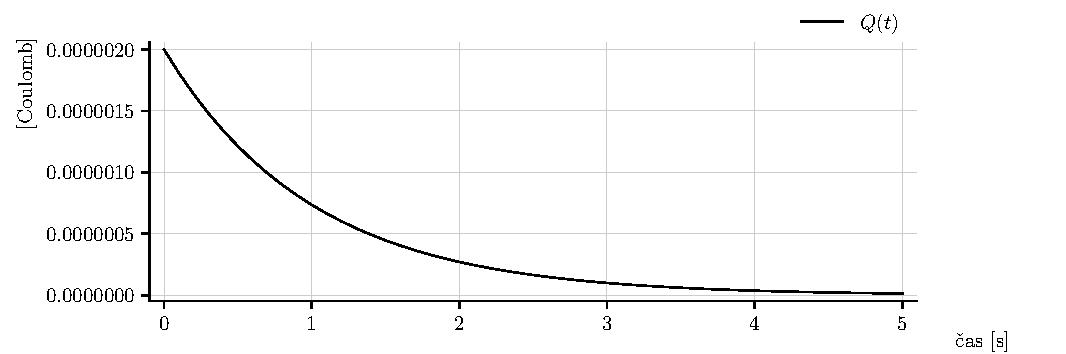
\includegraphics{../fig/cv01_fig_1.pdf}
	}

	\caption{Graf funkcie \eqref{rawRies2} pre $R = 10^6$ [$\Omega$], $C = 1$ [$\mu$F] a $Q_0 = 2\cdot 10^{-6}$ [Coulomb] (ľubovolné hodnoty len ako príklad)}
	\label{Graffunkcie}
\end{figure}




\subsubsection{Časový priebeh napätia na kondenzátore}


Vyšetrili sme časový priebeh elektrického náboja počas vybíjania kondenzátora. Opis situácie na začiatku časti~\ref{castVybij} však nepriamo predpokladá, že sa budeme venovať napätiu. Vzájomný vzťah už poznáme, a jeho formálne presnejší zápis (napätie $u(t)$ ako signál) je
\begin{equation} \label{QUsig}
    u(t) = \frac{1}{C} Q(t)
\end{equation}
Takže ak poznáme priebeh $Q(t)$, poznáme aj priebeh $u(t)$.

Začiatočnú podmienku pre signál $Q(t)$, teda hodnotu $Q(0)$ samozrejme tiež možno určiť so želanej (danej) začiatočnej podmienky signálu $u(t)$.
\begin{equation}
    Q(0) = C u_0
\end{equation}



\bigskip

\noindent
V zmysle úvodu časti~\ref{castVybij} uvažujme nasledujúci príklad
\begin{align*}
    C &= 1 \text{ [$\mu$F]} \\
    R &= 10^6  \text{ [$\Omega$]} \\
    u_0 &= 5  \text{ [V]}
\end{align*}
Pre tento príklad je následne začiatočná podmienka pre signál $Q(t)$
\begin{equation}
    Q(0) = 10^{-6} \cdot 5 = 0.000050 \text{ [Coulomb]}
\end{equation}
Výsledný priebeh napätia je zobrazený na obr.~\ref{PriebehNapatieDefault}.


\begin{figure}[!ht]
	\centering

	\makebox[\textwidth][c]{%
	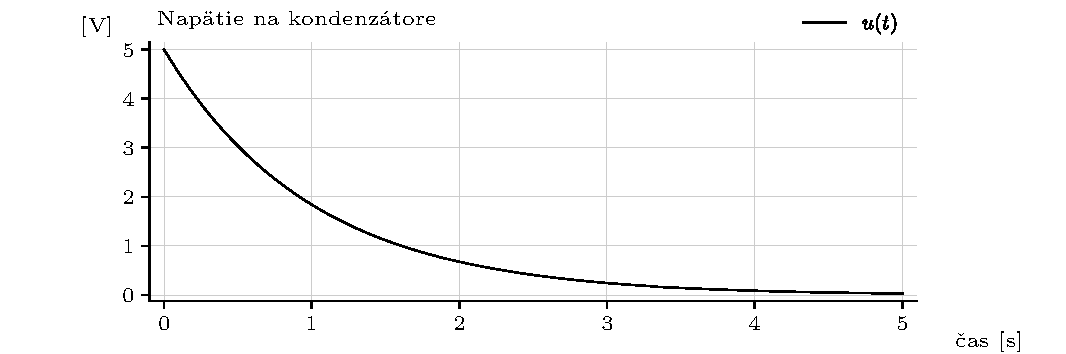
\includegraphics{../fig/cv01_fig_2.pdf}
	}

	\caption{Časový priebeh napätia na kondenzátore}
	\label{PriebehNapatieDefault}
\end{figure}







\subsubsection{Príklady pre rôzne parametre $R$ a $C$}


Pre zaujímavosť, ukážme priebeh napätia pre rôzne parametre $R$ a $C$. Príklady sú sumarizované v tabuľke~\ref{Príklady rôznych parametrov}. Graficky znázornené časové priebehy na obr.~\ref{PriebehNapatiePriklady}.


\begin{table}[!ht]
	\centering

	\caption{Príklady rôznych parametrov}
	\label{Príklady rôznych parametrov}

	\begin{tabular*}{\textwidth}{  l @{\extracolsep{\fill}} ccc }
		\toprule
            & $C$ [F] & $R$ [$\Omega$] & $u_0$ [V] \\
        \midrule
		Príklad 1 & $ 2 \cdot 10^{-6}$  & $10^{6}$  & 5 \\
		\midrule
		Príklad 2 & $\frac{1}{2} \cdot 10^{-6}$ & $10^{6}$  & 5 \\
		\midrule
		Príklad 3 &  $10^{-6}$ &  $ \frac{1}{10} \cdot 10^{6}$ & 3 \\
		\bottomrule
	\end{tabular*}
\end{table}


\begin{figure}[!ht]
	\centering

	\makebox[\textwidth][c]{%
	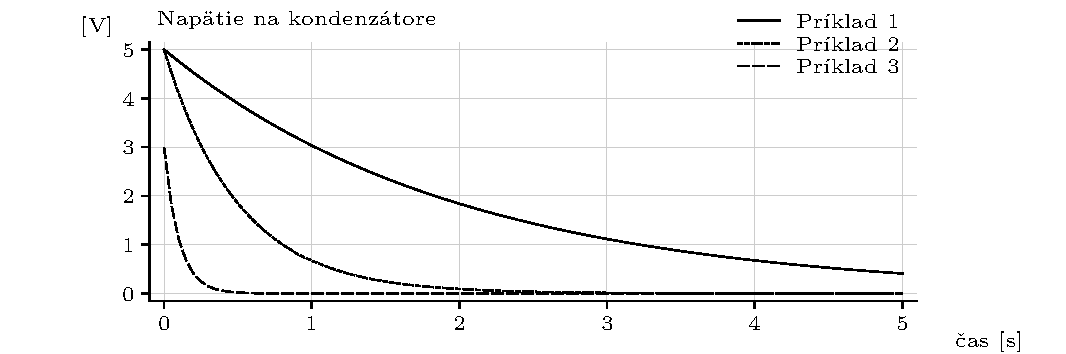
\includegraphics{../fig/cv01_fig_3.pdf}
	}

	\caption{Časový priebeh napätia na kondenzátore}
	\label{PriebehNapatiePriklady}
\end{figure}












\end{document}
